\documentclass[12pt,letterpaper]{article}
%%% LuaLaTex
\usepackage{fontspec}
\usepackage{amsmath}% if desired
\usepackage{unicode-math}
\renewcommand{\boldsymbol}{\symbf}

\setmainfont{TeX Gyre Pagella}[
Numbers	=	{OldStyle, Proportional},
Ligatures	=	TeX,
%Script=Arabic
%Contextuals = WordFinal,	
]
\setsansfont{TeX Gyre Adventor}[
Numbers	=	{OldStyle, Proportional},
Ligatures	=	TeX,
Scale=MatchLowercase]
\setmonofont{Inconsolata}[
Scale = MatchLowercase, 
Ligatures = TeX,
]
\setmathfont{Asana Math}
\setmathfont[range=it->up]{Neo Euler}
\setmathfont[range=up/{num}]{Neo Euler}
\newfontface{\andm}{Andale Mono}
\newfontface{\babm}{BabelStone Mayan Numerals}%{Symbola}
\newfontface{\mayanumerals}{BabelStone Mayan Numerals}
\newfontface{\charis}{Charis SIL}%{Gentium Plus}
\newfontface{\charisbf}{Charis SIL Bold}%{Charis SIL}
%\newfontface{\palarab}{PalatinoLTArabic}%{Gentium Plus}
%%%%%%%%%%%%
\linespread{1.05}% Palatino needs more leading (space between lines) {1.01} {1.08}
%\usepackage{ucs}
\usepackage[spanish,mexico]{babel}
%\usepackage{amsmath}
%\usepackage{amsfonts}
%\usepackage{amssymb}
%\usepackage{makeidx}
\usepackage{xcolor}
\usepackage{graphicx}
\usepackage[useregional]{datetime2}
\usepackage{fancyhdr}
\usepackage{tikz}
\usepackage[colorlinks=true,urlcolor=brown]{hyperref}
% % % %Geometry
\usepackage{geometry}%\usepackage[showframe]{geometry}
%\usepackage{layout}
\setlength{\voffset}{-0.7in}
\setlength{\headsep}{10pt}
\setlength{\textheight}{10.5in}
\usepackage{wasysym} %emoticons :)
%\usepackage[oldstyle]{kpfonts}
%\usepackage[T1]{fontenc}
\newcommand{\fej}{\relax\hfill\ifmmode{\lower.5ex\hbox{{\textcolor{blue}{\LARGE\smiley al 15pt}}}}\else\lower.5ex\hbox{{\textcolor{blue}{\LARGE \smiley}}}}  % Smiley emoticon :)
\author{\textsc{Manuel López Mateos}}
%%% 1° de noviembre de 2019
% % % % % % % Para usar título, autor y fecha por separado.
\makeatletter
\let\newtitle\@title
\let\elautor\@author
\let\newdate\@date
\makeatother
%
%
% % % % Enviroments
\newenvironment{definition}[1][Definición.]{\begin{trivlist}
\item[\hskip \labelsep {\bfseries #1}]}{\end{trivlist}}
% % % % % % % % % % % %
%
% % % % % % % % Headers
\pagestyle{fancy}
\fancyhf{}
\rhead{\color{olive}\hfill \DTMnow}
\lhead{\color{olive}\elautor}
\cfoot{\thepage}
\renewcommand{\headrule}{\color{olive}\hrule}
\newcommand{\R}{\relax\ifmmode\mathbb{R}\else${\mathbb{R}}$\fi}
%\rfoot{}
% % % % % % %
\begin{document} %\layout
%\noindent{\color{purple} \elautor \hfill \DTMnow
%\smallskip
%
%\hrule}
\bigskip 

\noindent Encuentra la \emph{\color{purple}intersección} de las rectas $f$ y $g$ en el plano $\R^2$,
$$f\colon\, y=2x+2,\qquad g\colon\, y=-3x+7$$

\begin{figure}[ht]
\centering
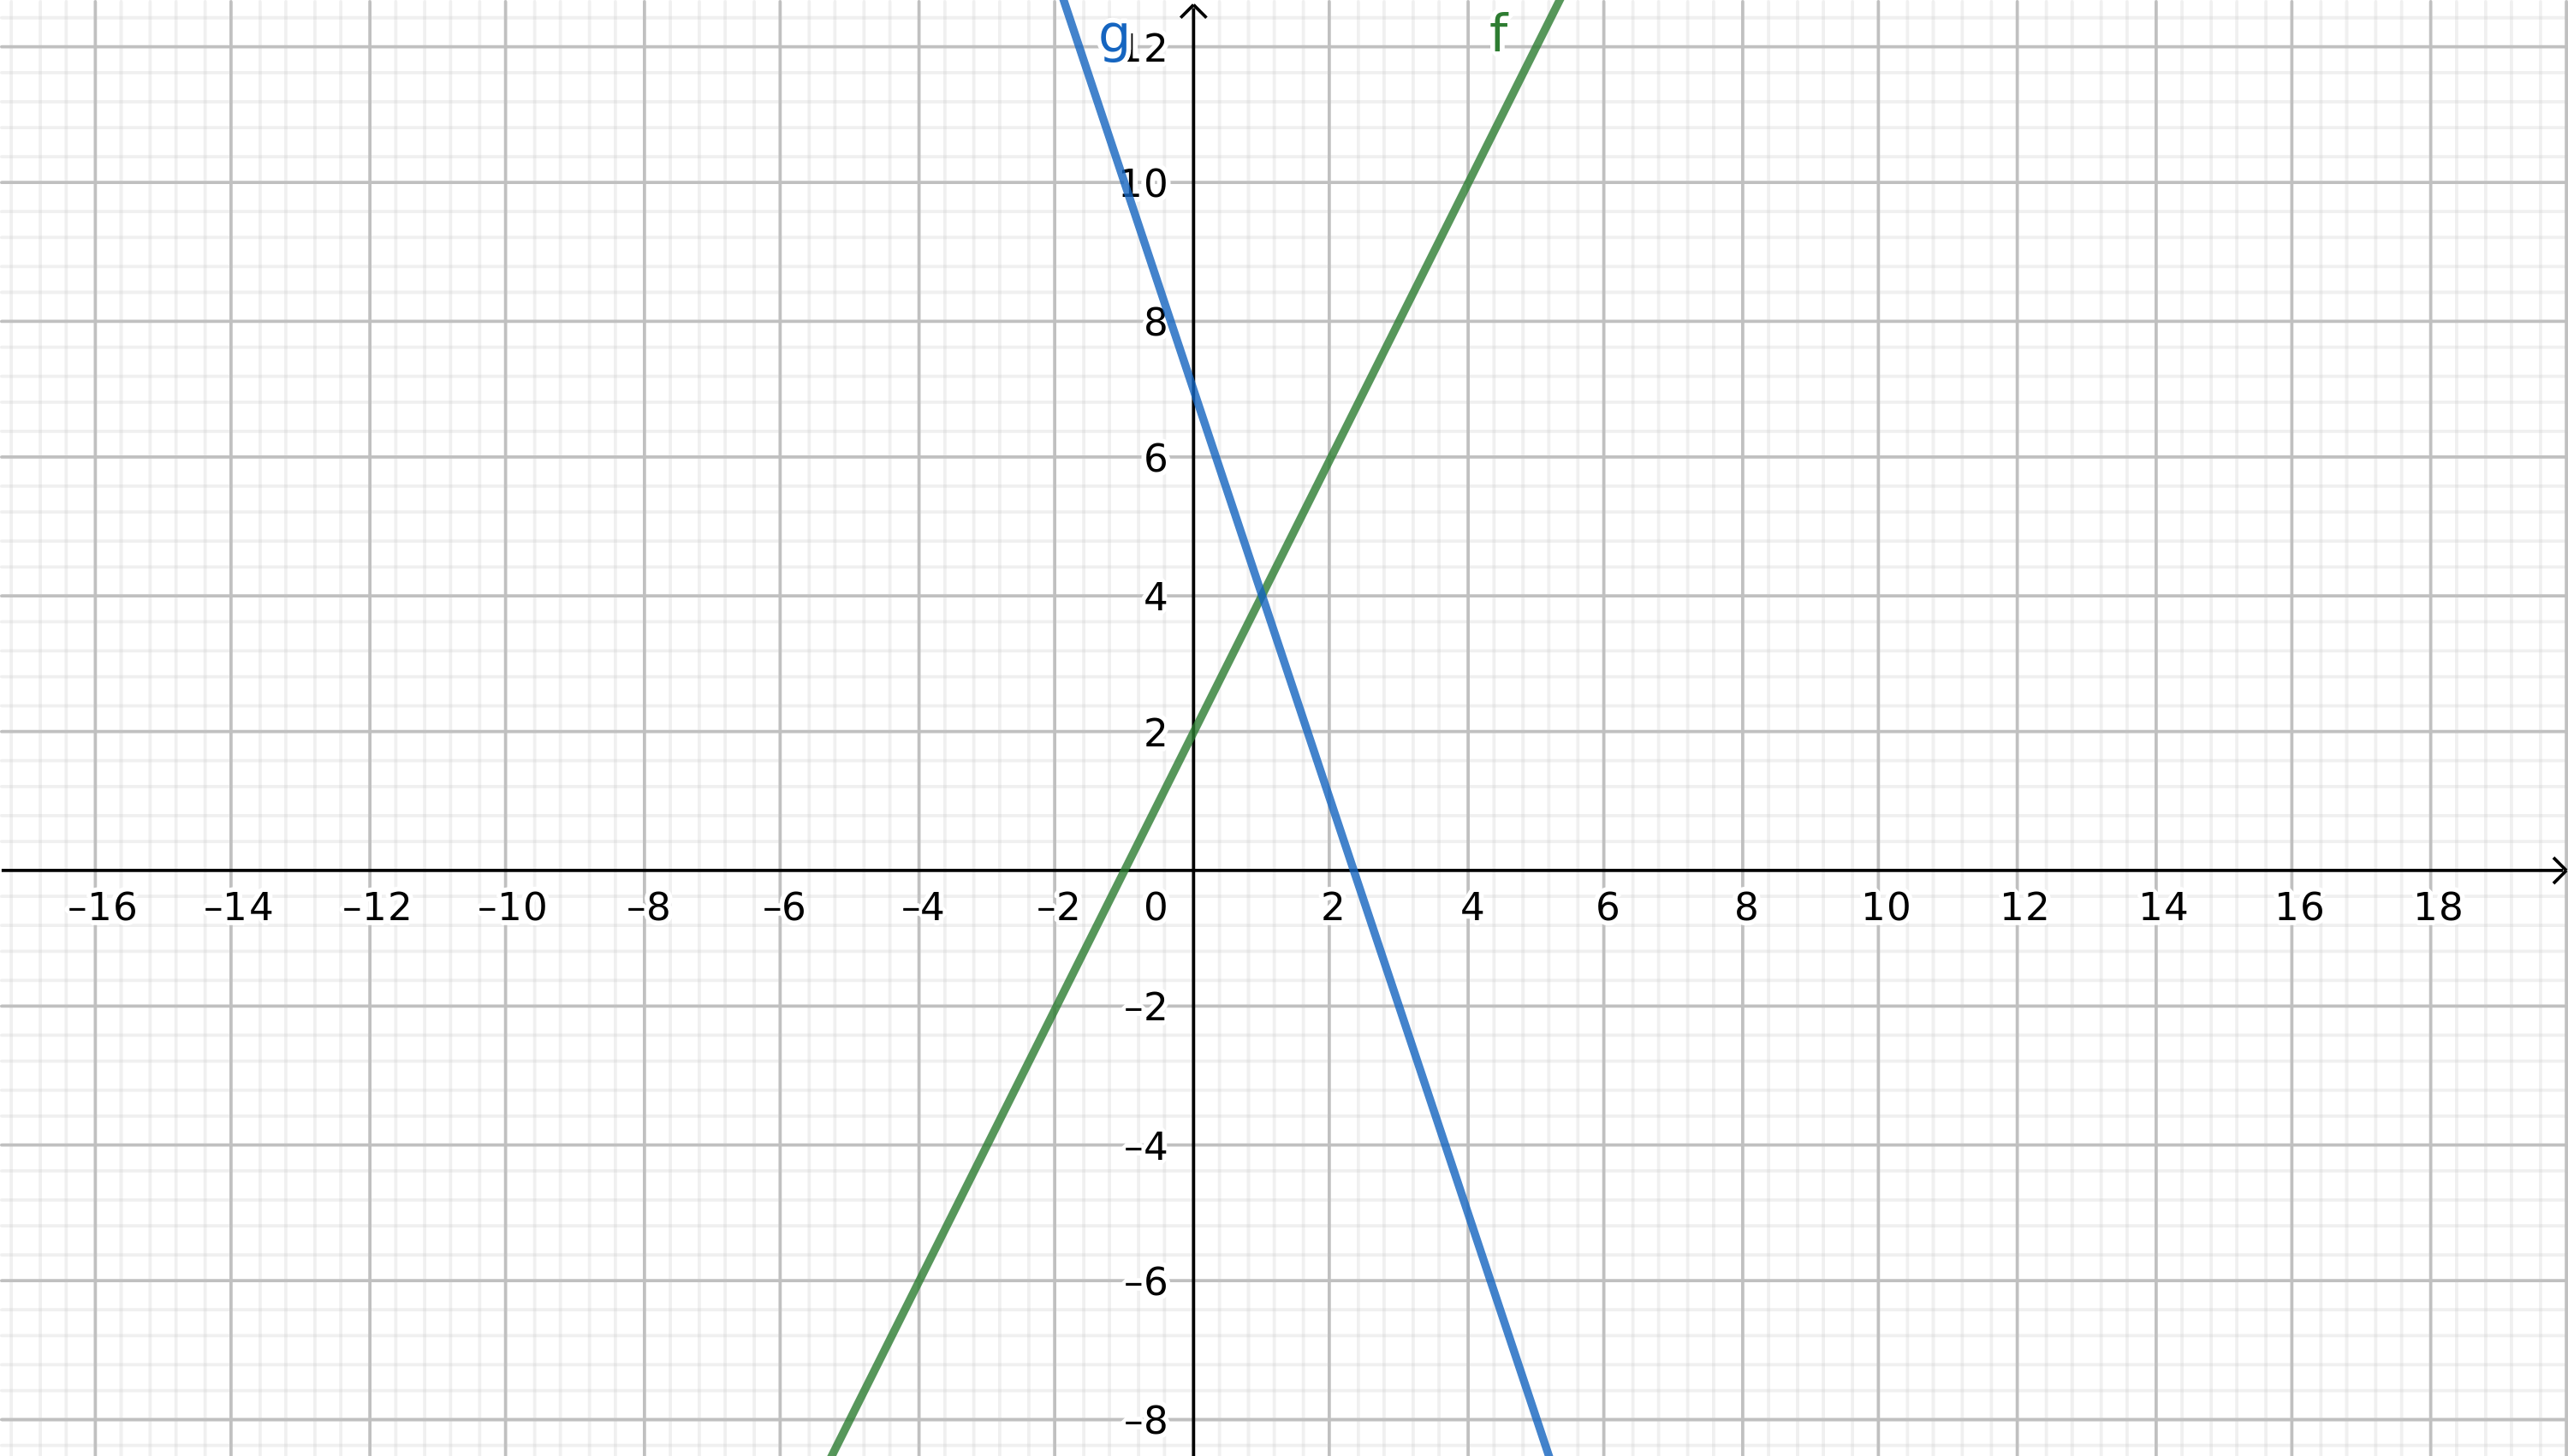
\includegraphics[scale=0.31]{img/intersec-rectas.png}
\caption{En verde la gráfica de $y=2x+2$, en azul la gráfica de $y=-3x+7$.}\label{fig:interrec}
\end{figure}

Las coordenadas $(p_1,p_2)$ del punto de intersección $P$ de las rectas $f$  y $g$, deben satisfacer ambas ecuaciones, es decir
\begin{align}
p_2&=2p_1+2,\\
p_2&=-3p_1+7.
\end{align} 

Una manera de resolver el anterior \emph{\color{purple}sistema de ecuaciones}, dos \emph{ecuaciones} con dos \emph{incógnitas}, a saber $p_1$ y $p_2$, es:
\begin{quotation}
	\noindent Despejar $p_2$ en la ecuación (1) ---de hecho ya lo está---, substituir el resultado en la ecuación (2), despejar de ahí $p_1$, obteniendo su \emph{\color{purple}valor}. Lo substituimos en cualesquiera de las dos ecuaciones para hallar el \emph{valor de $p_2$}.
\end{quotation}


Al substituir $p_2$ en la ecuación (2) obtenemos
$$2p_1+2=-3p_1+7$$
(lo que equivale a \emph{igualar ambas ecuaciones}) despejamos $p_1$,
\begin{align*}
2p_1+3p_1&=7-2\\
5p_1&=5\\
p_1&=\frac{5}{5}=1.
\end{align*}
Es decir, $p_1=1$. Substituimos este valor en la ecuación (1),
\[p_2=2p_1+2=2(1)+2=4.\]

Así, el punto de intersección de las rectas $f$ y $g$ es $P=(1,4)$.

\fej
\vfill 

\begin{center}
	{\footnotesize\color{olive} Esta hoja se formó con el sistema \LaTeX. La gráfica con \textsc{Geogebra}, \url{https://www.geogebra.org/}}
\end{center}
\end{document}